\documentclass{article}

\usepackage{enumerate}
\usepackage[bottom=1in,top=1in]{geometry}
\usepackage{parskip}
\usepackage{graphicx}
\usepackage{subcaption}
\usepackage[pdftex,colorlinks,urlcolor=blue]{hyperref}

\geometry{letterpaper}

\begin{document}

\title{CS376 PA3 Report}

\author{
  Jiawei Yao\\
  \texttt{jwyao@stanford.edu}
  \and
  Wei Wei\\
  \texttt{wwei2@stanford.edu}
}

\maketitle

\section{Task 1 - Cosine Similarity}

Parameters and NDCG of train and dev datasets:

\begin{table}[!htb]
    \centering
    \begin{tabular}{ | l | l | l | l | l | l |}
    \hline
    \textbf{Param} & $c_{anchor}$ & $c_{body}$ & $c_{header}$ & $c_{title}$ & $c_{url}$ \\
    \hline
    \textbf{Value} & 1.00 & 3.19 & 4.40 & 4.35 & 4.30 \\
    \hline
    $\mathbf{NDCG_{train}}$ & \multicolumn{5}{c|}{0.8651} \\
    \hline
    $\mathbf{NDCG_{dev}}$ & \multicolumn{5}{c|}{0.8508} \\
    \hline
    \end{tabular}
    \caption{Parameters for Task 1}
\end{table}

\textbf{Tuning Strategy} Initially we randomly select value from $[0,5]$ for each parameter and compute NDCG train and dev set respectively\footnote{See \texttt{RandomTuner.java}.}. After normalizing the values by $c_{anchor}$, We found that with $c_{anchor}= 1.00, c_{body}\approx 1.60, c_{head}\approx 3.60, c_{title}\approx4.30, c_{url}\approx4.60$, NDCG $> 0.8670$ can be achieved on train set. On the other hand, with $c_{anchor}= 1.00, c_{body}\approx 3.40, c_{head}\approx 3.60, c_{title}\approx4.80, c_{url}\approx4.60$, NDCG $> 0.8515$ can be achieve on dev set. Then we narrow down the range for each parameter and manually tuned the paramters to get satisfactory NDCG on both sets. The final parameter value and result is in the table above.

\textbf{Reasonings behind the Weights} First, the weights for header, title and url fields are larger than that of body. This aligns with intuition because header and title contains summary information of the document. When a query term appearing in header or title, it is highly likely that the document is relevant to the query. The reasoning for url is similar. This is the same reason why human readable url is good for SEO. Second, it might be strange that anchor weight is the lowest at a first look. This is actually the result of multiplying by the anchor count -- raw term frequency is anchor field tends to be larger than term frequency in other fields.

We made the following design choices in cosine scorer:

\begin{itemize}
    \item We use body\_length + 500 to do length normalization. The actual value of added length doesn't seem to matter so much so we stick to 500 as suggested.
    \item Sublinear scaling is \emph{NOT} used on raw document term frequencies as it turns out with sublinear scaling the performance degrades.
\end{itemize}

\section{Task 2 - BM25F}

\begin{table}[!htb]
  \centering
  \begin{tabular}{ | l | l | l | l | l | l |}
    \hline
    \textbf{Param} & $B_{anchor}$ & $B_{body}$ & $B_{header}$ & $B_{title}$ & $B_{url}$ \\
    \hline
    \textbf{Value} & 0.20 & 1.00 & 0.50 & 0.90 & 1.00 \\
    \hline
    \textbf{Param} & $W_{anchor}$ & $W_{body}$ & $W_{header}$ & $W_{title}$ & $W_{url}$ \\
    \hline
    \textbf{Value} & 1.60 & 0.10 & 1.60 & 3.10 & 3.00 \\
    \hline
    \textbf{Param} & $K_1$ & $\lambda$ & $\lambda'$ & \multicolumn{2}{c|}{} \\
    \hline
    \textbf{Value} & 2.50 & 1.60 & 2.10 & \multicolumn{2}{c|}{}\\
    \hline
    $\mathbf{NDCG_{train}}$ & \multicolumn{5}{c|}{0.8919} \\
    \hline
    $\mathbf{NDCG_{dev}}$ & \multicolumn{5}{c|}{0.8829} \\
    \hline
  \end{tabular}
  \caption{Parameters for Task 2}
\end{table}

\textbf{Tuning Strategy} We use local hill climbing with random restart to tune the parameter. To achieve good performance on both training data set and dev data set, we manually adjust the parameter we get from local hill climbing tuning algorithm.

In Hill Climbing algorithm, we define the neighbors of a candidate to be as follows:
\begin{itemize}
  \item First select a parameter type to tune. Get the range of that parameter.
  \item Then generate candidates with other parameters unchanged, only changes that parameter's value.
\end{itemize}

\textbf{Reasonings behind the Weights}:

\begin{itemize}
  \item \textbf{url:} $W_{url}$ is $3.0$ which is the second largest (only a little smaller than $W_{title}$). Url has large weights makes sense becuase url often contains crucial information about this page. In fact, when I evaluated the query relevance myself, I found that url is very can tell us a lot about what this page is about. $Bf_{url}$ is $1.0$. It also makes sense because for these two urls \url{http://nlp.stanford.edu/manning/tex/} and \url{http://nlp.stanford.edu/manning/tex/avm.sty} and the query is \textit{christopher manning latex macros}, the former urls is shorter than the latter while the former contains all the key word of the latter. The latter may be more specific and contains less information of our information need.
  \item \textbf{title:} $W_{title}$ is $3.1$ which is the largest. Title has the largest weight is reasonable becuase title summarizes the contents of a web document. $Bf_{title}$ is $0.9$. It is reasonable because longer title may contain more specific information about a specific event. For example, our query is \textit{ wilbur dining}, there are a page whose title is \textit{when logging into webmail a no authentication error message displays stanford answers} and another page whose title is \textit{http://answers.stanford.edu/category/email-and-calendar/webmail}. The latter provides a better answer for user's information need because the former contains authentication error which the user didn't want to know.
  \item \textbf{body:} $W_{body}$ is only $0.1$ which is the lowest. Body is very long and may cover a lot of words in the query. The weight is low because term frequency in body is very high and we don't want body to be the most important factor in scoring documents. $Bf_{body}$ is $1.0$ and it is reasonable because if one document has long body length but has the same body hits as a shorter document, the shorter document tends to be more relevant than the longer document.
  \item \textbf{header:} $W_{header}$ is $1.6$ which has the same weight as anchor but much smaller than title and url. Header often suggests the content overview of a paragraph. Some paragraph may not be related to user's information need so the total weight given to header is not that high as title and url. $Bf_header$ is $0.5$.
  \item \textbf{anchor:} $W_{anchor}$ is $1.6$. Anchor text tells us a lot but anchor count is often very large and the anchor in other website may not summarizes the core idea of the web document so the weight is not that high as title and url but it is much more important than body. $Bf_{anchor}$ is 0.2 which suggests that the length of the anchor text is not very important to the query relevance. The length of anchor text varies a lot: some anchor has a very large count so that the lenght of anchor text is very long. We don't want these to affect the scoring of our BM25F scorer so the value is only 0.2.
\end{itemize}


\section{Task 3 - Smallest Window}

Our smallest window scorer is based on cosine similarity scorer. Parameters and NDCG of train and dev datasets:

\begin{table}[!htb]
    \centering
    \begin{tabular}{ | l | l | l | l | l | l | l |}
    \hline
    \textbf{Param} & $B$ & $c_{anchor}$ & $c_{body}$ & $c_{header}$ & $c_{title}$ & $c_{url}$ \\
    \hline
    \textbf{Value} & 2.65 & 1.00 & 3.19 & 4.40 & 4.35 & 4.30 \\
    \hline
    $\mathbf{NDCG_{train}}$ & \multicolumn{6}{c|}{0.8675} \\
    \hline
    $\mathbf{NDCG_{dev}}$ & \multicolumn{6}{c|}{0.8521} \\
    \hline
    \end{tabular}
    \caption{Parameters for Task 3}
\end{table}

\textbf{Tuning Strategy} We applied a tuning strategy similar to that used in tunining cosine similarity scorer. The preliminary result showed that, with different parameter configuration, the overall improvement is not so obvious. As a result, we fix $c_*$ parameters from cosine similarity scorer and took effort to tune parameter $B$.

We used three different boost functions ($\frac{1}{x}$, $\frac{1}{x^2}$ and $e^{-x}$) and tried $B$ in range $[1.0, 10.0]$ with step $0.01$. The result is plotted as follows:

\begin{figure}[!htb]
  \centering
  \begin{subfigure}{.3333\textwidth}
      \centering
      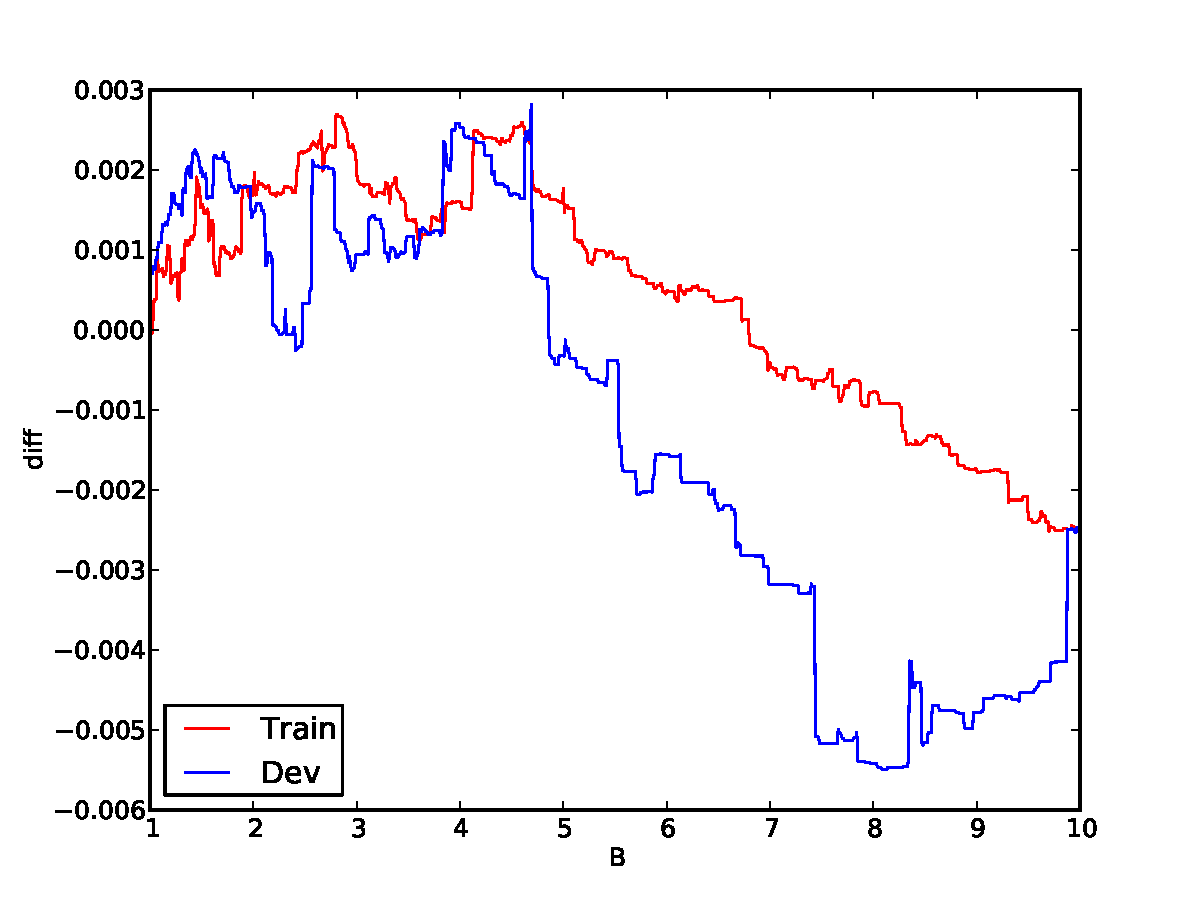
\includegraphics[width=\linewidth]{sw.pdf}
      \caption{Gain of NDCG with $\frac{1}{x}$}
      \label{fig:diff-inverse}
  \end{subfigure}%
  \begin{subfigure}{.3333\textwidth}
      \centering
      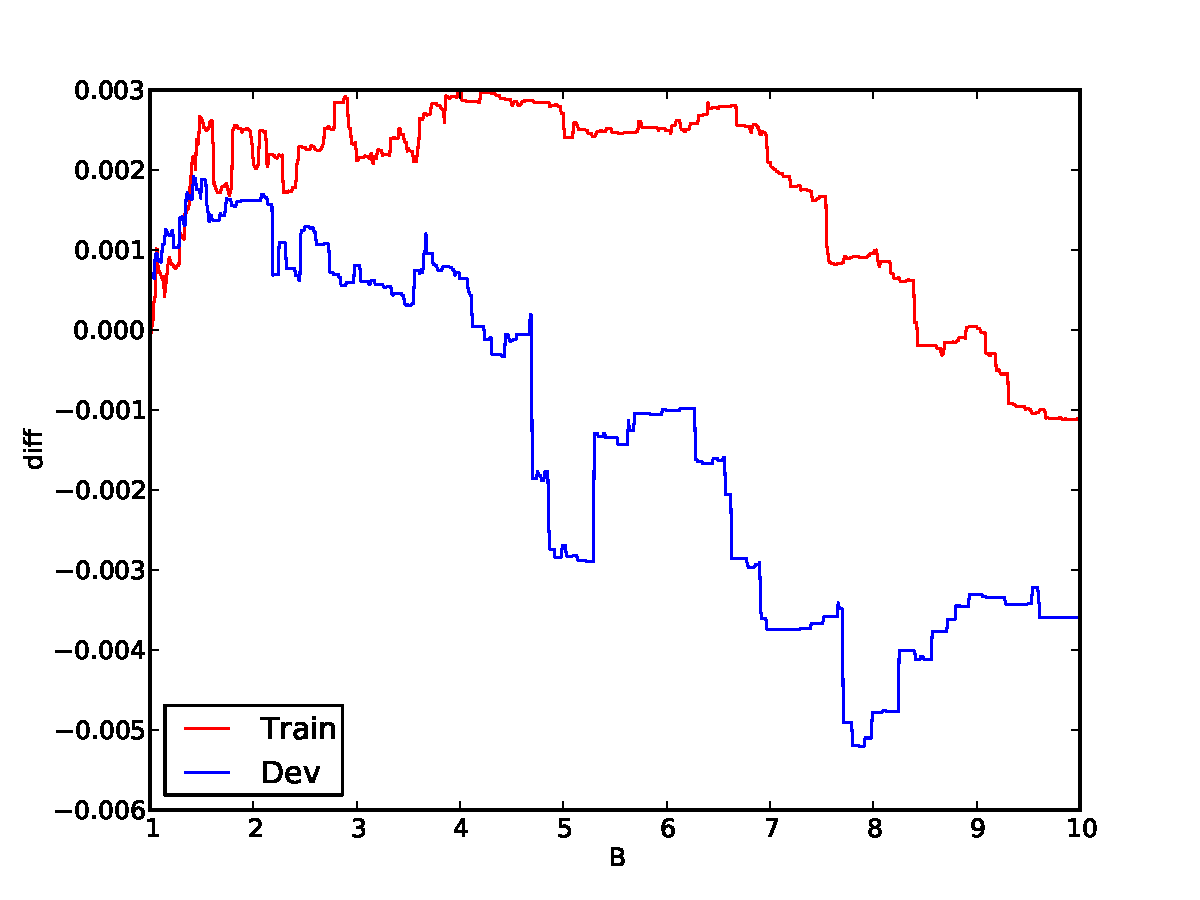
\includegraphics[width=\linewidth]{sw-square.pdf}
      \caption{Gain of NDCG with $\frac{1}{x^2}$}
      \label{fig:diff-square}
  \end{subfigure}%
  \begin{subfigure}{.3333\textwidth}
      \centering
      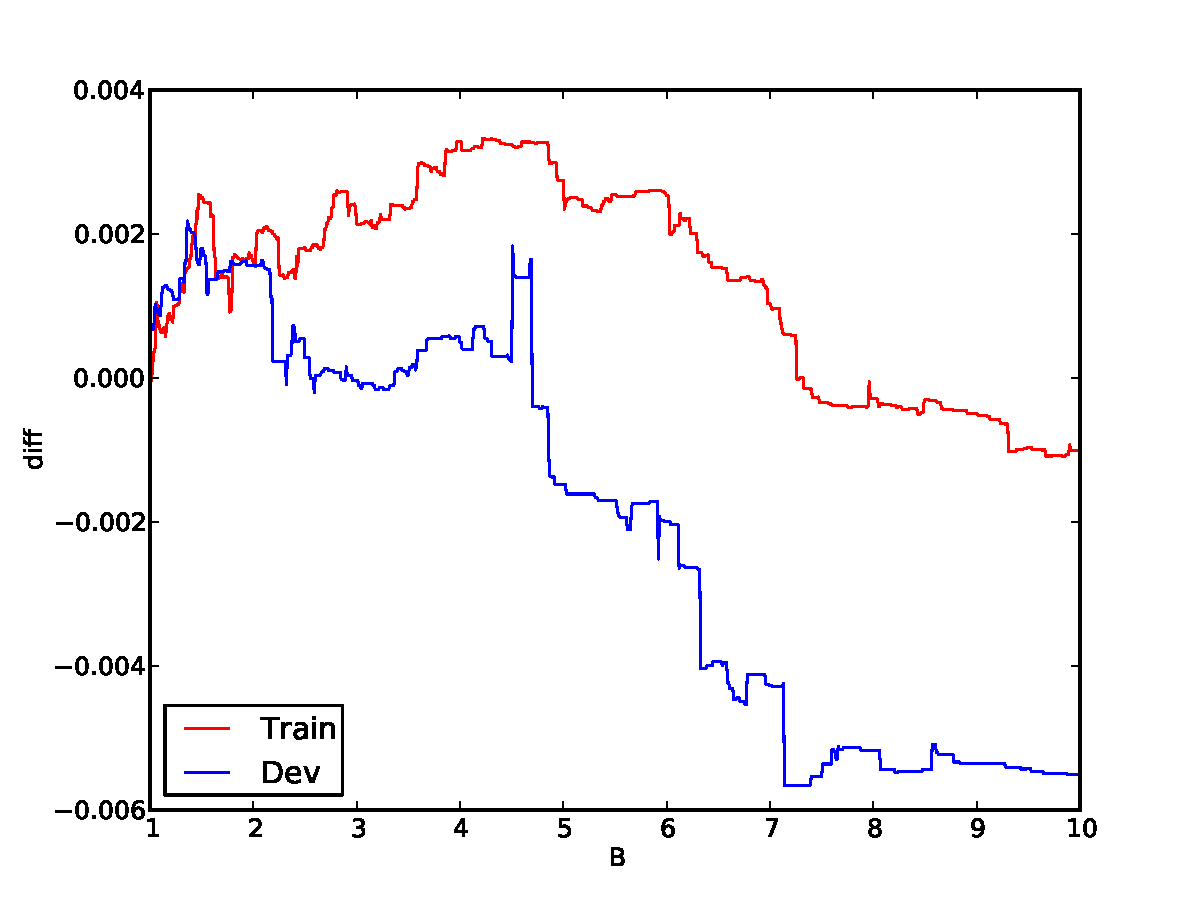
\includegraphics[width=\linewidth]{sw-exp.pdf}
      \caption{Gain of NDCG with $e^{-x}$}
      \label{fig:diff-exp}
  \end{subfigure}
  \caption{Tuning $B$}
  \label{fig:tune-b}
\end{figure}

In each plot, the x-axis is value of $B$ and the y-axis is the difference from NDCG values achieved in cosine similarity scorer achieved in Task 1. We can see that with whichever boost function and $B<5$, we can gain a improvement of NDCG on both train and dev sets. However, different behaviors emerge with different boost functions with $B<5$:

\begin{itemize}
    \item With $\frac{1}{x}$, the trend of NDCG gain is generally similar for both sets. Moreover, there're local maxima for both train and test sets at $B\approx 2.6$ and $B\approx 4.6$.
    \item With $\frac{1}{x^2}$, there's no coherent trend for the two sets. While NDCG for train set keeps a gain of $0.02$+, the gain for test set is generally decreasing.
    \item With $e^{-x}$, the NDCG gain for train set is the best of the three functions, with a maximum over 0.03. At $B\approx 4.6$, both sets get a local maximum gain. However, the gain for dev set is not as good as that of $\frac{1}{x}$'s.
\end{itemize}

As a result, we chose $\frac{1}{x}$ as the boost function and $B=2.65$ as the parameter.

\textbf{Reasons behind the Parameters} The argument for $c_*$ is similar to that in Task 1. For $B$, intuitively, it should not be too large as it serves only as a boost factor and the smallest window is not a very good indicator of relevance. The figures confirm this with extra large $B$ hurting performance. But for small B, there's really not a big difference. For $\frac{1}{x}$, it turns out that several values of $B$ can achieve a similar boost so our choice here is just a result of data.

\section{Q\&A}

\paragraph{Question 1}
What was the reasoning behind giving the weights to the url, title, body, header and anchor fields for the three tasks? Were there any particular properties about the documents that allowed a higher weight to be given to one field as opposed to another?

\vspace{-3mm}
\paragraph{Solution 1}
The reasoning with the choice of different weights for each scorer is discussed in previous sections. As with the properties of documents, as we observed, the average length of body is extremely large ($> 3000$), which is three orders of magnitude larger than that of url, title or header. As a result, a query term appearing in the latter three fields is much more informative than appearing in body. Hence the weights for url, title and header is larger. The anchor field is special because a corresponding count is multiplied, which gives it a larger average length and decreases its weight. There might be other interesting properties of document structure, but with the limited format of given data, unfortunately it's hard to probe.

\paragraph{Question 2}
What other metrics, not used in this assignment, could be used to get a better scoring function from the document? The metrics could either be static (query-independent, e.g. document length) or dynamic (query-dependent, e.g. smallest window).

\vspace{-3mm}
\paragraph{Solution 2}
Static metrics such as time of creation may help to achieve a better scoring function from the document. Sometimes we may type in a time in the query string to find an article, time of creation may help a lot if we include time in the metric.

Dynamic metrics like user interests, author, location may help too. User interests is a very import feature. If I type in Jordan, and I search AI a lot, the search engine should return Jordan in UC Berkeley. Author may also be helpful because if we want to find Andrew Ng's paper, including author in the metric may help us find better result. Location is becoming more and more important. If I type in restaurant, it is better to return restaurant near your location. Query click information may also be very useful. Click information aggregated across many users signals the relevance of the document and the query.

\paragraph{Question 3}
In BM25F, in addition to the weights given to the fields, there are 8 other parameters, $B_{url}$, $B_{title}$, $B_{header}$, $B_{body}$, $B_{anchor}$, $\lambda$, $\lambda'$ and $K_1$. How do these parameters affect the ranking function?

\vspace{-3mm}
\paragraph{Solution 3}
The reasoning behind $B_{url}$, $B_{title}$, $B_{header}$, $B_{body}$, $B_{anchor}$ is shown in section 2. Please refer to section 2 for details.

We find our choices of $K_1$, $\lambda$ and $\lambda'$ through our local hill climbing algorithm. They works great for both train data set and dev data set.

\paragraph{Question 4}
In BM25F, why did you select a particular $V_j$ function?

\vspace{-3mm}
\paragraph{Solution 4}
We choose $\log (\mbox{pagerank} + \lambda')$ as $V_j$ function. It is similar to a saturation function in that a document with pagerank score 1 may be much worse than a document with a pagerank score 2 but a document with pagerank score 8 is similar to a document with score 9. As long as the document's pagerank score is not very low we should not penalize it much.

We use $\log$ function also because this function is used in pratice and it has fairly good performance.

\paragraph{Question 5}
For a function that includes the smallest window as one component, how does varying $B$ and the boost function change the performance of the ranking algorithm?

\vspace{-3mm}
\paragraph{Solution 5}
This problem is discussed in Task 3. To conclude, $B$ should not be too large and different boost functions have similar general behavior. Also, adding such boost to Cosine Similarity Scorer doesn't help improve performance very much.

\end{document}
